\subsection{Feynman Rules in $\phi ^ 4 $ theory} 

When we consider interaction terms which contain 
the same species of particle, things get a bit more complicated, 
and we need to take into account different permutations we can get. 
When considering something like the 
Yukawa interaction, $ H _ I =  g \int d^ 3 x \psi \psi ^ * \phi $, 
our interaction term contains distinct particles. That means, for example, 
that our Feynman rules we derived earlier doesn't come 
with extraneous factors and we only have to add a prefactor $ ( - ig ) $
at each vertex point. 
However, for the case of an interacting theory like 
 \[
 \mathcal{ H } _ I = \frac{\lambda }{ 4 ! } \phi ^ 4  
\] we have to change our thinking a bit for the sake of making life 
easier. On might think that, similar to the above case, 
that a vertex drawn in the Feynman rules for $ \phi ^ 4 $ theory 
might mean that we add a factor of $ \frac{ - i \lambda }{ 4 ! } $, 
however, taking into account the different permutations
of the four $ \phi $ fields, it's easier for us to just 
attach a $  - i \lambda $ for each vertex then divide by a small number 
based on the look of the diagram. 
Our final goal here will be to compute amplitudes which contain 
terms like 
\[
 i \mathcal{ M } \sim \frac{ - i \lambda}{ 4 ! } \int d^ 4 x \, 
 \bra{ p_1 ' , p_2 ' } : \phi ( x) \phi ( x) \phi ( x) \phi ( x) \ket{ p_1 , p_2 } 
\]

\subsubsection{Combinatoric factors} 
To motivate our discussion, we'll start by considering interactions 
in position, and not momentum space. We'll start by calculating 
a propagator-like object for a scattering system with $ m $ particles, 
which is given by 
\[
 \bra{ 0 } \mathcal{ T } \left\{  \phi_1 \dots \phi _n S  \right\} \ket{ 0 } 
\] In our perturbation expansion for the case of $ \phi ^ 4 $ theory, 
we'll have terms like 
\[
	\frac{1}{n ! } \left( \frac{- i \lambda }{ 4 ! }  \right)^ n 
	\int d^ 4 y_1 \dots d^ 4 y_n \bra{ 0 } T \left\{ \phi_1 \dots \phi _n 
	 \phi ^ 4 ( y _ 1 ) \dots \phi ^ 4 ( y _ n ) \right\} \ket{ 0 }  
\] To illustrate the idea of symmetry factors, we will consider the 
case of a first order expansion ($ n  = 1$), with 
four particles to consider. We expand our integral as 
\[
	\dots = \frac{ - i \lambda  }{ 4 } \int d ^ 4 x 
	\bra{ 0 } \mathcal{ T } \left\{  \phi _ 1 \dots \phi_4 \phi_x ^ 4  \right\} \ket{ 0 }  
\] Now, we apply Wick's theorem to determine 
the non-vanishing components in the integrand. One possible 
configuration we could have is that we could contract 
each of the $ \phi _ i $ term s with one 
of the $ \phi_ x$ terms, which gives several terms up to permutation. 
Or we could contract two of the $ \phi _ i $ ' s together 
and contract the rest with $ \phi _ x $. Finally, we could have 
also just contracted the $ \phi _ i $'s amongst themselves, and t
the  $ \phi _ x $ 's amongst themselves. In total, this sum then looks like 
\begin{align*}
	\dots &=  \frac{ - i \lambda }{ 4 ! } \int d^ 4 x \, 
	 \wick{\c1 \phi _ 1 \c2 \phi _ 2 \c3 \phi _ 3 \c4 \phi_4 \c1
\phi _ x \c2 \phi _ x \c3 \phi _ x \c4 \phi _ x}\\
 & + \text{ similar terms gained from contracting all }  \phi _ i \text{ with } \phi _ x \\
 & + \frac{ - i \lambda }{ 4 ! } \int d ^ 4 x \, 
 \wick{ \c1 \phi_1 \c1 \phi_ 2 \c1 \phi _ 3 \c2 \phi _ 4 
 \c1 \phi_ x \c2 \phi _ x \c1 \phi _ x \c1 \phi _ x } \\
 & + \text{ similar contractions which only contract two }  \phi _ x  \\ 
  & +  \frac{ - i \lambda }{ 4 ! }  \int d^ 4 x \, 
  \wick{ \c \phi _ 1 \c \phi _ 2 \c \phi _ 3 \c \phi _ 4 
  \c \phi _ x \c \phi _ x \c \phi _ x \c \phi _ x } \\
  & + \text{  similar contractions where no } \phi _ x \text{ is contracted with }
  \phi _ i 
\end{align*}
Now, the upshot of this is that since contractions are $ \mathbb{ C} $ functions, 
Each of the terms in the same 'category' yield the same expression in 
terms of Feynman propagators. For the first term, we have a total 
of $ 24 $  permutations that yield the above. This is because we can 
contract $ \phi _ 1 $ with any of the $4  $ $ \phi _x $ 's. Then, we can 
pair $ \phi_ 2 $ with the remaining $ 3 $ , and so on. So we have $ 4 ! $ permutations here.
Each of these terms yields a factor of 
\[
\frac{ - i \lambda }{ 4!} \int d ^ 4 x \, \Delta_ F ( x_1 - x ) \Delta_ F( x_2  - x) \Delta_ F ( x_3 - x ) 
\Delta _ F( x_4 - x ) 
\] and since we have 24 of them, our total contribution is 
\[
- i \lambda \int d ^ 4 x \, \Delta _ F ( x_1 - x ) \Delta_ F ( x_2 - x ) \Delta _ F( x_3 - x ) 
\Delta _ F ( x_4 - x) 
\] Now, looking \textbf{specifically} at the terms where we have 
$ \phi _ 3 $ and $ \phi _ 4 $ contracted with $ \phi _ x $, 
we have $ 12 $ ways to configure our contractions. More so, we
could have equally included terms which contracted 
$ \phi _ 1 $ and $ \phi _ 2 $ with $ \phi  _ x $ instead, which again 
yields a term with $ 12 $ contractions (we have 6 possible
diagrams which give this configuration, each of them 
implcitly summing over $12 $ possibilities). 
Finally, in the term where we contract $ x_ 1 $ with $ x_ 2 $, 
and $ x_3 $ with $ x_ 4 $, we have 3 possible ways for 
the  $ \phi _ x 's $ to contract amongst themselves. 

Thus, our total expansion in terms of Feynman propagators 
is given by 
\begin{align*}
	 \bra{ 0 } T \left\{  \phi _ 1 \phi _ 2 \phi _ 3 \phi _ 4 \phi _ x 
	 \phi _ x \phi _ \phi x \right\}  \ket{ 0 }  &=   - i \lambda \int d ^ 4 x \Delta _ F ( x_ 1- x ) 
	 \Delta _ F ( x_ 2 - x ) \Delta _ F ( x_ 3 - x ) \Delta _F ( x_4 - x ) \\
	  &  \frac{ -i  \lambda }{ 2 } \int d ^ x \Delta _ F ( x_1 - x_2 ) 
	 \Delta _ F ( x_3  - x ) \Delta _ F ( x_4 - x ) \Delta _ F ( x- x) \\
	  &  + \text{ 5 similar permutations } \\
	  & - \frac{ i \lambda }{ 8 } \int d ^ 4 x \Delta _ F ( x_1 - x_2) \Delta _ F ( x_3 - x_4) 
	  \Delta_ F ( x - x) \Delta _ F ( x - x ) \\
	  & + \text{ 2 similar permuations}
\end{align*}

\begin{figure}[h]
	\centering
	\includegraphics[width=0.8\linewidth]{figures/phifour.pdf}
	\caption{A diagrammatic expansion of 
	our representation}%
	\label{fig:}
\end{figure} 

Now, if we expand to higher order, to $ O ( \lambda ^ 2 ) $,
we might get a term like 
 \[
	 \frac{1}{2 } \left(  \frac{ - i \lambda }{ 4 ! }  \right)  ^ 2 
	 \int d ^ 4 x d ^ 4 y \bra{ 0 } T \left\{  
	 \phi _ 1 \phi_2 \phi_3 \phi_4 \phi _ x ^ 4 \phi _ y ^ 4 \right\}  \ket{ 0 } 
\]  Now, in this term, if we 
insist that $ x_1 $ and $ x_2 $ are contracted with 
$ \phi _ x $ and that $ \phi _ 3 , \phi _ 4 $ are contracted 
with $ \phi  _ y $, then we could get a contraction 
that looks like
\[
  \wick{\c1 \phi _ 1 \c 2 \phi _ 2 \c 3 \phi _ 3 \c 4 \phi _ 4 
	  \c  1 \phi _ x \c 2 \phi _ x \c 5 \phi _ x 
	  \c 6 \phi _ x \c 6 \phi _ y \c 3 \phi _ y 
  \c 5 	\phi _ y \c 4 \phi _ y } 
\] Now we ask how many terms of this type there are. 
We have a total of 12 possibilities from our possible 
contractions of $ \phi _ 4 , \phi _ 3 $ with $ \phi _ y $. 
And, we also have 12 times this from  $ \phi_1 , \phi _ 2 $ 
with $ \phi _ x $. This means that our prefactor 
is going to be 
\[
 \frac{1}{2 } = \frac{1}{2 } \frac{1}{ 4 ! } 12 \times 12 
\] Our associated diagram for this kind of object 
is shown in figure \ref{fig:phiFourSecond}. 

\begin{figure}[h]
	\centering
	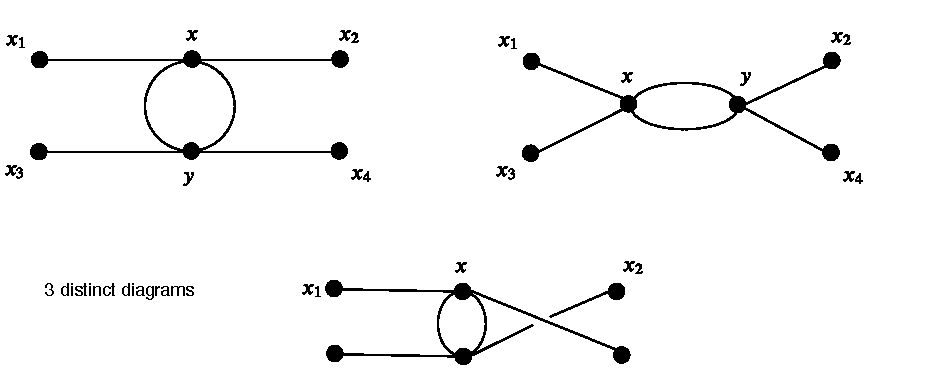
\includegraphics[width=0.8\linewidth]{figures/phiFourSecond.pdf}
	\caption{All diagrams of the above type with distinct 
	contractions; each has a symmetry factor of 2}%
	\label{fig:phiFourSecond}
\end{figure}
Our associated contribution to this scattering 
in terms of Feynman propagators is then 
\[
	\frac{ ( - i \lambda ) ^ 2 }{ 2 } \int d^ x \, d ^ 4 y \, 
	\Delta _ F ( x_1 - x ) \Delta _ F ( x_2 - x ) 
	\Delta _ F ( x_3 - y ) \Delta _ F ( x_4 - y ) 
	 ( \Delta _ F ( x - y ) ) ^ @
\]

\subsubsection{Deriving our Feynman rules} 
We can now use our analysis above to 
match a diagram with an integral expression. 
We conclude that the expression 
\[
 \bra{ 0 } T \left\{  \phi _ 1 \dots \phi _ m 
 \exp \left(  \frac{ - i \lambda }{ 4 ! } \int d ^ 4 x \phi ^ 4 _ x  \right) \right\} \ket{ 0 }  
\]  is the sum off all possible diagrams with $ m $ 'external points' 
which are just points with a single line coming out of them, along 
with any number of internal vertex points (which are points with 
four lines coming into them since we are dealing with $ \phi ^ 4 $ theory. 
Our routine is to then, for each diagram that exists, have the Feynman rules where we 
\begin{enumerate}
	\item Attach a propagator $ \Delta _ F ( x -y ) $ for any 
		line connecting the points $ x $ and $ y $, no matter 
		whether they represent external or internal points. 
	\item For every vertex (a point where four lines meet), this 
		represents an integral over our interaction space 
		so we ascribe a factor of $ ( - i \lambda ) \int d ^ 4 x $. 
	\item We divide by the appropriate symmetry factor of the diagram. 
\end{enumerate}
Now, we have a nice way to write down amplitudes in $ \phi ^ 4 $ theory 
in position space. The next thing to do would then 
be to transfer this into some momentum rules. Recall our momentum 
expansion of the Feynman propagator 
\[
	D _ F ( x - y ) = \int \frac{ d ^  4 p }{ ( 2 \pi ) ^ 4 } \frac{i }{ p ^ 2 
	- m ^ 2  + i \epsilon } e ^{ - i p \cdot  ( x - y ) }
\] This integral has a nice interpretation. Since this represents a line going 
from $ y $ into $ x $, we interpret $ e ^{ i  p \cdot  y } $ and 
$ e ^{  - i p \cdot  x }$ as momentum factors we can attach at 
each vertex for momentum going out of $ y $ and into $ x $. In addition, 
our  $ \frac{i}{ p ^ 2 - m ^ 2 _ i \epsilon } $ factor can be 
an expression attached to the line itself. 
At a vertex point, we'll have some propagators coming in 
to meet at a point. Due to the fact that we're integrating 
over $ \int d ^ 4 x $ , a factor like this corresponds to 
\[
	\int d ^ 4 x e ^{  -i x \cdot  ( p_1 + p_2 - p_3 - p_4 ) } = 
	( 2 \pi ) ^ 4 \delta ^ 4 ( p_1 + p_2 - p_3 - p_4 ) 
\] for example. Hence, in momentum space, 
our Feynman rules look like 
\begin{enumerate}
	\item For each line, assign a momentum $ p $ and attach 
		a factor of $ \frac{i}{p ^ 2 - m ^ 2 + i \epsilon } $
		in the integral. 
	\item At each vertex, assign a factor of $ i \lambda $, 
		and also impose the conservation of momentum which 
		comes from a delta function appearing. 
	\item Integrate over all other undetermined momenta 
		$ \int \frac{ d ^ 4 k}{  ( 2 \pi ) ^  4}$ 
	\item Divide by the symmetry factor of the diagram 
\end{enumerate}

\subsubsection{Vacuum Bubbles and Connected Diagrams} 
If we consider scattering both to and from our 
free theory vacuum state, we are describing the term 
$ \bra{ 0 } S \ket{ 0 }  $. This means however, 
that we have no external points. Our only valid diagrams 
are the ones where every point is an internal vertex (four lines 
going in). So, our total amplitude 
is given by the sum of all vacuum bubble diagrams
shown in figure \ref{fig:vacuumExpand}.  
\begin{figure}[htpb]
	\centering
	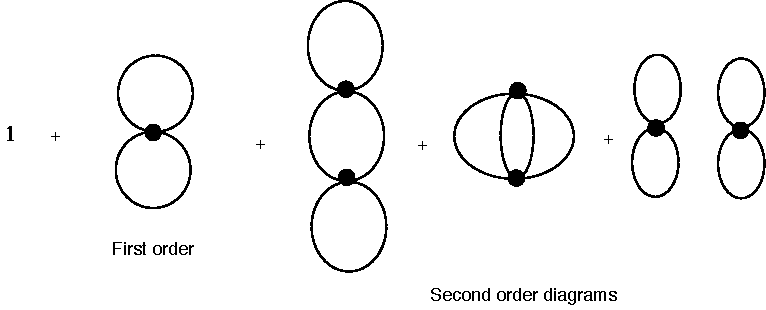
\includegraphics[width=0.8\linewidth]{figures/vacuumExpand.pdf}
	\caption{All vacuum bubble diagrams contributing 
	to the scattering}%
	\label{fig:vacuumExpand}
\end{figure}
Now, one can convince themselves that we can write 
this sum as an exponential of just distinct vacuum bubble diagrams. 
This sum is shown diagrammatically in figure \ref{fig:fourvac}. 
\begin{figure}[h]
	\centering
	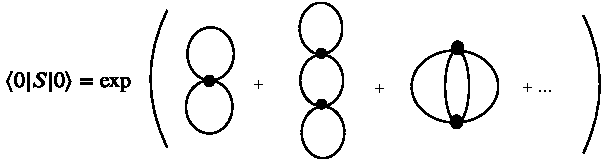
\includegraphics[width=0.8\linewidth]{figures/PhiFourVacuumExp.pdf}
	\caption{Combinatoric factors work out to give an exponential 
	of distinct vacuum types}%
	\label{fig:fourvac}
\end{figure}
In other words, we can write our vacuum amplitude as 
\[
	\bra{ 0 } S \ket{ 0 } = \exp \left(  \text{Distinct vacuum bubble types} \right) 
\] 
Now, from our previous discussion, we had that a term like 
\[
 \bra{ 0 } T \left\{  \phi _ 1 \dots \phi _ n   S \right\}  \ket{ 0 } = \sum \text{ 
 diagrams with m external points}
\]  but, amazingly, we have that this quantity \textbf{factorizes}
into two parts, one factor being the exponential of 
distinct vacuum bubble types $ \bra{ 0 } S \ket{ 0 } $, 
and the other factor the sum of just connected diagrams. 
\[
	\bra{ 0 } T \left\{  \phi _ 1 \dots \phi _ m S  \right\} \ket{ 0 } = 
	\left(  \sum \text{ connected diagrams }  \right) \left(  \bra{ 0 } S \ket{ 0 }  \right) 
\]  
